\chapter{Introduction to Cyber-Physical Systems}
\label{ch:introduction}
\index{cyber-physical systems|(}

% Learning objectives:
% - Understand what cyber-physical systems are and their key characteristics
% - Appreciate the role of model-based development in CPS engineering
% - Recognize why control engineers need real-time systems knowledge
% - Understand why software engineers need control systems knowledge
% - See how the four modules of this course connect

\section{The Challenge of Flying Robots}

Consider a quadrotor\index{quadrotor} hovering in your living room. To the casual observer, it appears to float effortlessly, making tiny adjustments to maintain its position. But beneath this apparent simplicity lies an extraordinary engineering challenge that spans multiple disciplines.

Every two milliseconds---five hundred times per second---the following sequence must complete:

\begin{enumerate}
    \item \textbf{Sense}: Read accelerometer, gyroscope, and barometer data from the IMU
    \item \textbf{Estimate}: Fuse noisy sensor readings into a coherent estimate of orientation and velocity
    \item \textbf{Compute}: Calculate the control commands needed to track the desired trajectory
    \item \textbf{Actuate}: Send PWM signals to the four motors
\end{enumerate}

If any step takes too long, arrives late, or produces incorrect results, the quadrotor falls. There is no graceful degradation---gravity is unforgiving.

\begin{center}
\begin{tikzpicture}[every node/.style={font=\small}]
    % Timeline
    \draw[thick, -{Stealth}] (0,0) -- (12,0) node[right] {time};

    % 2ms markers
    \foreach \x in {0, 4, 8} {
        \draw[thick] (\x, -0.15) -- (\x, 0.15);
    }
    \node[below] at (0, -0.2) {$0$};
    \node[below] at (4, -0.2) {$2$ ms};
    \node[below] at (8, -0.2) {$4$ ms};

    % Control cycle
    \fill[blue!30] (0.1, 0.3) rectangle (0.6, 0.8);
    \fill[green!30] (0.6, 0.3) rectangle (1.4, 0.8);
    \fill[orange!30] (1.4, 0.3) rectangle (2.2, 0.8);
    \fill[red!30] (2.2, 0.3) rectangle (2.6, 0.8);

    \fill[blue!30] (4.1, 0.3) rectangle (4.6, 0.8);
    \fill[green!30] (4.6, 0.3) rectangle (5.4, 0.8);
    \fill[orange!30] (5.4, 0.3) rectangle (6.2, 0.8);
    \fill[red!30] (6.2, 0.3) rectangle (6.6, 0.8);

    % Legend
    \fill[blue!30] (0, -1) rectangle (0.4, -0.7);
    \node[right] at (0.5, -0.85) {Sense};
    \fill[green!30] (2, -1) rectangle (2.4, -0.7);
    \node[right] at (2.5, -0.85) {Estimate};
    \fill[orange!30] (4.5, -1) rectangle (4.9, -0.7);
    \node[right] at (5, -0.85) {Compute};
    \fill[red!30] (7.5, -1) rectangle (7.9, -0.7);
    \node[right] at (8, -0.85) {Actuate};

    % Deadline arrow
    \draw[dashed, red!60] (4, 0) -- (4, 1.2);
    \node[above, red!60] at (4, 1.2) {Deadline};
\end{tikzpicture}
\end{center}

What makes this problem so challenging is that it requires expertise from multiple engineering disciplines simultaneously:

\begin{itemize}
    \item \textbf{Control theory}: Designing controllers that stabilize an inherently unstable system
    \item \textbf{Signal processing}: Filtering noisy sensor data and fusing multiple measurements
    \item \textbf{Real-time systems}: Ensuring computations complete within strict deadlines
    \item \textbf{Embedded software}: Implementing algorithms efficiently on resource-constrained hardware
    \item \textbf{Verification}: Testing that the system behaves correctly under all conditions
\end{itemize}

No single discipline provides all the answers. A control engineer who designs a beautiful controller on paper may find it unstable when implemented due to computational delays. A software engineer who writes elegant code may inadvertently break the timing assumptions that the control design depends on. A verification engineer who tests only the software may miss failures that emerge from the interaction between code and physics.

\begin{keyidea}
Cyber-physical systems require engineers who can work across the boundaries of control theory, computer science, and electrical engineering. This course teaches you to be that kind of engineer.
\end{keyidea}

\section{What Are Cyber-Physical Systems?}

The term \emph{cyber-physical systems}\index{cyber-physical systems|textbf} (CPS) was coined by Helen Gill at the National Science Foundation in 2006 to describe systems where computational and physical processes are deeply intertwined. Unlike traditional embedded systems that merely monitor or control physical processes, CPS are characterized by tight, bidirectional coupling between computation and physics.

\begin{definition}[Cyber-Physical System]
A \textbf{cyber-physical system} is an engineered system where computational algorithms and physical processes are integrated such that each affects the other through feedback loops, and correctness depends on both the logical behavior of software and the dynamic behavior of physical components.
\end{definition}

\subsection{Key Characteristics of CPS}

Several characteristics distinguish cyber-physical systems from traditional software or control systems:

\paragraph{Tight Coupling of Computation and Physics}
In CPS, the computational elements do not merely observe the physical world---they actively shape it, and the physical world shapes the computation in return. The quadrotor's motors change its orientation, which changes what the sensors measure, which changes what the controller computes, which changes the motor commands. This closed loop operates continuously, with each domain affecting the other.

\paragraph{Real-Time Constraints}
\index{real-time constraints}
CPS must respond to physical events within bounded time. A late response is often as bad as a wrong response. If the quadrotor's attitude controller runs 10\% slower than designed, the control loop becomes unstable---not because the algorithm is wrong, but because timing is part of correctness.

\paragraph{Concurrency and Distribution}
\index{concurrency}
CPS typically involve multiple computational tasks running concurrently, often on distributed processors. The quadrotor runs sensor fusion, attitude control, position control, and communication tasks simultaneously, and these tasks must coordinate without interfering with each other.

\paragraph{Safety Criticality}
\index{safety criticality}
Many CPS operate in contexts where failures have serious consequences. Autonomous vehicles, medical devices, and industrial robots can cause physical harm if they malfunction. This demands rigorous approaches to design, implementation, and verification that go beyond typical software engineering practices.

\paragraph{Heterogeneity}
CPS integrate diverse components: analog sensors, digital processors, mechanical actuators, communication networks, and human operators. Each component has its own characteristics, failure modes, and constraints that must be understood and managed.

\subsection{CPS Examples Beyond Quadrotors}

While this course uses the quadrotor as a running example, cyber-physical systems are ubiquitous in modern technology:

\begin{itemize}
    \item \textbf{Automotive}: Engine control, anti-lock braking, adaptive cruise control, autonomous driving. Modern vehicles contain 50--100 electronic control units (ECUs) coordinating thousands of functions.

    \item \textbf{Aerospace}: Flight control systems, autopilots, engine management. Aircraft like the Boeing 787 are ``fly-by-wire''---the pilot's inputs are interpreted by computers that send commands to control surfaces.

    \item \textbf{Medical devices}: Pacemakers, insulin pumps, surgical robots. These systems directly affect human health and must meet stringent safety requirements.

    \item \textbf{Power systems}: Smart grids balance electricity generation and consumption across millions of nodes in real-time, integrating renewable sources with varying output.

    \item \textbf{Manufacturing}: Industrial robots, CNC machines, and automated production lines require precise coordination of multiple axes and processes.

    \item \textbf{Building systems}: HVAC control, lighting, security systems increasingly operate as integrated CPS, optimizing energy use while maintaining comfort.
\end{itemize}

\subsection{The Interdisciplinary Challenge}

CPS exist at the intersection of multiple engineering disciplines, as illustrated in Figure~\ref{fig:cps-intersection}.

\begin{figure}[htbp]
\centering
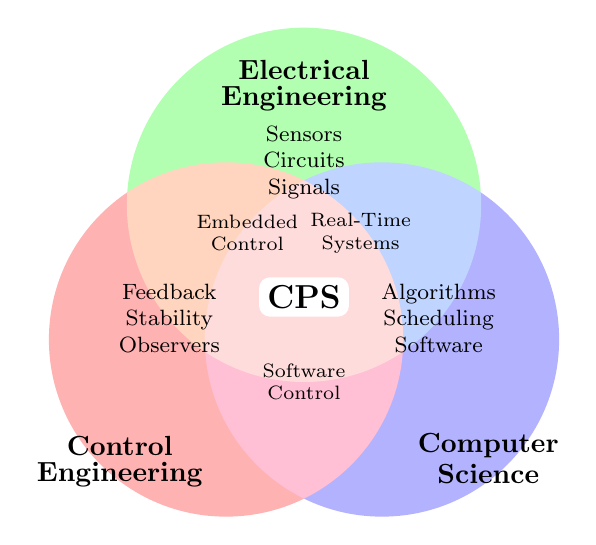
\begin{tikzpicture}[scale=0.9]
    % Three overlapping circles
    \begin{scope}[blend group=soft light]
        \fill[red!30] (0,0) circle (2.5cm);
        \fill[blue!30] (2.2,0) circle (2.5cm);
        \fill[green!30] (1.1,1.9) circle (2.5cm);
    \end{scope}

    % Labels outside
    \node[font=\bfseries] at (-1.5, -1.5) {Control};
    \node[font=\bfseries] at (3.7, -1.5) {Computer};
    \node[font=\bfseries] at (-1.5, -1.9) {Engineering};
    \node[font=\bfseries] at (3.7, -1.9) {Science};
    \node[font=\bfseries] at (1.1, 3.8) {Electrical};
    \node[font=\bfseries] at (1.1, 3.4) {Engineering};

    % Topics in each region
    \node[font=\footnotesize, align=center] at (-0.8, 0.3) {Feedback\\Stability\\Observers};
    \node[font=\footnotesize, align=center] at (3, 0.3) {Algorithms\\Scheduling\\Software};
    \node[font=\footnotesize, align=center] at (1.1, 2.5) {Sensors\\Circuits\\Signals};

    % CPS in the center
    \node[font=\bfseries\large, fill=white, rounded corners, inner sep=3pt] at (1.1, 0.6) {CPS};

    % Pairwise intersections
    \node[font=\scriptsize, align=center] at (0.3, 1.5) {Embedded\\Control};
    \node[font=\scriptsize, align=center] at (1.9, 1.5) {Real-Time\\Systems};
    \node[font=\scriptsize, align=center] at (1.1, -0.6) {Software\\Control};
\end{tikzpicture}
\caption{Cyber-physical systems emerge at the intersection of control engineering, computer science, and electrical engineering. Effective CPS development requires fluency across these boundaries.}
\label{fig:cps-intersection}
\end{figure}

Historically, these disciplines developed largely independently, each with its own assumptions, tools, and culture:

\begin{itemize}
    \item \textbf{Control engineering} assumes continuous-time dynamics, ideal sensors, and instantaneous computation. Analysis focuses on stability, performance, and robustness using differential equations and transfer functions.

    \item \textbf{Computer science} abstracts away physical timing, focusing on logical correctness, computational complexity, and software architecture. Real-time is often treated as a specialized concern.

    \item \textbf{Electrical engineering} deals with analog signals, noise, power constraints, and hardware interfaces. The focus is on circuits, signal integrity, and electromagnetic compatibility.
\end{itemize}

CPS engineering requires integrating insights from all three disciplines. This is more than superficial knowledge---it requires understanding how decisions in one domain affect the others. Choosing a faster sampling rate (control decision) increases computational load (software impact) and power consumption (hardware impact). Using a cheaper sensor (hardware decision) increases noise (signal processing impact) and may require a more conservative controller (control impact).

\begin{notebox}
This course is designed to develop fluency across these disciplines. You will learn not just the techniques from each field, but how to reason about their interactions when building real systems.
\end{notebox}

\section{Model-Based Development}
\index{model-based development|(}

\subsection{What is Model-Based Development?}

Traditionally, engineering development follows a document-centric approach: requirements are written in documents, designs are described in documents, and implementation is done by programmers reading those documents. This creates several problems:

\begin{itemize}
    \item Documents are ambiguous and incomplete
    \item Translation from documents to code introduces errors
    \item There is no automated way to verify consistency
    \item Changes require updating multiple documents and code manually
\end{itemize}

\textbf{Model-based development}\index{model-based development|textbf} (MBD) addresses these problems by making executable models---not documents---the central artifacts throughout the development process.

\begin{definition}[Model-Based Development]
\textbf{Model-based development} is a software and systems engineering approach where mathematical and computational models serve as the primary artifacts for specifying, analyzing, designing, and implementing systems. Models are not just documentation---they are executable specifications that can be simulated, analyzed, and automatically translated into implementation code.
\end{definition}

The key insight is that a model is both a specification and an implementation draft. When you create a Simulink\index{Simulink} model of an attitude controller, you are simultaneously:

\begin{enumerate}
    \item Specifying what the controller should do (the mathematical relationship between inputs and outputs)
    \item Creating something that can be simulated to verify behavior
    \item Providing a source from which implementation code can be generated
\end{enumerate}

\subsection{The Model-Based Development Workflow}

Figure~\ref{fig:mbd-workflow} shows the typical workflow in model-based development.

\begin{figure}[htbp]
\centering
\begin{tikzpicture}[
    node distance=2cm,
    stage/.style={draw, rectangle, rounded corners, minimum width=2.8cm, minimum height=1.2cm, align=center, font=\small},
    arrow/.style={-{Stealth}, thick}
]
    % Stages
    \node[stage, fill=blue!15] (req) {Requirements\\Capture};
    \node[stage, fill=green!15, right of=req, xshift=1.5cm] (model) {System\\Modeling};
    \node[stage, fill=yellow!15, right of=model, xshift=1.5cm] (sim) {Simulation \&\\Analysis};
    \node[stage, fill=orange!15, right of=sim, xshift=1.5cm] (codegen) {Code\\Generation};
    \node[stage, fill=red!15, right of=codegen, xshift=1.5cm] (test) {Testing \&\\Verification};

    % Forward arrows
    \draw[arrow] (req) -- (model);
    \draw[arrow] (model) -- (sim);
    \draw[arrow] (sim) -- (codegen);
    \draw[arrow] (codegen) -- (test);

\end{tikzpicture}
\caption{The model-based development workflow. Models created early in development are refined and eventually used for code generation.}
\label{fig:mbd-workflow}
\end{figure}

\begin{enumerate}
    \item \textbf{Requirements Capture}: System requirements are captured in a structured form, often linked directly to model elements. Requirements traceability is maintained throughout development.

    \item \textbf{System Modeling}: Engineers create mathematical models of the plant (physical system) and the controller. These models capture the essential dynamics and control logic.

    \item \textbf{Simulation and Analysis}: Models are simulated to verify behavior before any hardware exists. Analysis tools check stability, performance, and safety properties.

    \item \textbf{Code Generation}: Production code is automatically generated from verified models. The generated code is structurally similar to the model, maintaining traceability.

    \item \textbf{Testing and Verification}: Generated code is tested at multiple levels---from software-in-the-loop (same code, simulated plant) to hardware-in-the-loop (real hardware, simulated environment) to full system testing.
\end{enumerate}

Crucially, the model remains the single source of truth throughout this process. When requirements change, engineers update the model, re-simulate, re-generate code, and re-test. The model ensures consistency across all stages.

\subsection{The V-Model and Testing Levels}

Model-based development is often organized using the \textbf{V-model}\index{V-model}, a development framework that pairs each design phase with a corresponding verification phase. Understanding the V-model is essential for planning verification activities and for understanding the testing levels used throughout this course.

\paragraph{The V-Model Framework}
The V-model gets its name from its shape: design activities descend on the left side, implementation occurs at the bottom, and verification activities ascend on the right side. Each design phase on the left has a corresponding test phase on the right:

\begin{center}
\begin{tikzpicture}[
    every node/.style={font=\small},
    phase/.style={draw, rectangle, rounded corners, minimum width=2.8cm, minimum height=0.7cm, align=center},
    arrow/.style={-{Stealth}, thick}
]
    % Left side - Design
    \node[phase, fill=blue!20] (req) at (0, 3) {Requirements};
    \node[phase, fill=blue!15] (arch) at (-1.5, 2) {Architecture};
    \node[phase, fill=blue!10] (design) at (-3, 1) {Detailed Design};
    \node[phase, fill=yellow!20] (impl) at (-3, 0) {Implementation};

    % Right side - Verification
    \node[phase, fill=green!20] (accept) at (6, 3) {Acceptance Test};
    \node[phase, fill=green!15] (sys) at (4.5, 2) {System Test};
    \node[phase, fill=green!10] (int) at (3, 1) {Integration Test};
    \node[phase, fill=orange!20] (unit) at (3, 0) {Unit Test};

    % Design flow
    \draw[arrow] (req) -- (arch);
    \draw[arrow] (arch) -- (design);
    \draw[arrow] (design) -- (impl);

    % Implementation to test
    \draw[arrow] (impl) -- (unit);

    % Test flow
    \draw[arrow] (unit) -- (int);
    \draw[arrow] (int) -- (sys);
    \draw[arrow] (sys) -- (accept);

    % Horizontal traceability
    \draw[dashed, gray] (req) -- (accept);
    \draw[dashed, gray] (arch) -- (sys);
    \draw[dashed, gray] (design) -- (int);

    % Labels
    \node[left of=design, xshift=-1cm, font=\footnotesize\itshape] {Design};
    \node[right of=int, xshift=1cm, font=\footnotesize\itshape] {Verify};
\end{tikzpicture}
\end{center}

The dashed horizontal lines show \emph{traceability}: requirements are verified by acceptance tests, architecture by system tests, and detailed design by integration tests. This structure ensures that every design decision has a corresponding verification activity.

\paragraph{Why the V-Model for CPS?}
The V-model is particularly valuable for cyber-physical systems:

\begin{itemize}
    \item \textbf{Traceability}: Each test verifies a specific design artifact. When a test fails, you know which design element is problematic.
    \item \textbf{Early planning}: Test strategies are defined during design, not as an afterthought. This prevents discovering untestable requirements late in development.
    \item \textbf{Certification}: Safety standards like DO-178C\index{DO-178C} (aerospace) and ISO~26262\index{ISO 26262} (automotive) require evidence of systematic verification at each level.
\end{itemize}

\paragraph{Testing Levels for Model-Based Development}
For model-based CPS development, the V-model's verification side is implemented through a progression of testing levels. Each level increases the amount of real hardware involved, trading speed for fidelity:

\begin{center}
\begin{tikzpicture}[
    every node/.style={font=\small},
    level/.style={draw, rectangle, rounded corners, minimum width=1.6cm, minimum height=1.4cm, align=center},
    arrow/.style={-{Stealth}, thick}
]
    % Testing levels
    \node[level, fill=blue!20] (mil) at (0, 0) {\textbf{MIL}\\Model-in-\\the-Loop};
    \node[level, fill=green!20] (sil) at (2.8, 0) {\textbf{SIL}\\Software-in-\\the-Loop};
    \node[level, fill=yellow!20] (pil) at (5.6, 0) {\textbf{PIL}\\Processor-in-\\the-Loop};
    \node[level, fill=orange!20] (hil) at (8.4, 0) {\textbf{HIL}\\Hardware-in-\\the-Loop};
    \node[level, fill=red!20] (vil) at (11.2, 0) {\textbf{VIL}\\Vehicle-in-\\the-Loop};

    % Arrows
    \draw[arrow] (mil) -- (sil);
    \draw[arrow] (sil) -- (pil);
    \draw[arrow] (pil) -- (hil);
    \draw[arrow] (hil) -- (vil);

    % Labels below - positioned clearly below the boxes
    \node[below of=mil, yshift=-0.3cm, font=\scriptsize, align=center] {All\\simulated};
    \node[below of=sil, yshift=-0.3cm, font=\scriptsize, align=center] {Code on\\host};
    \node[below of=pil, yshift=-0.3cm, font=\scriptsize, align=center] {Code on\\target};
    \node[below of=hil, yshift=-0.3cm, font=\scriptsize, align=center] {Full\\hardware};
    \node[below of=vil, yshift=-0.3cm, font=\scriptsize, align=center] {Real\\environment};

    % "More hardware" arrow spanning above all boxes
    \draw[arrow] (0, 1.5) -- (11.2, 1.5) node[midway, above, font=\small] {More hardware};
\end{tikzpicture}
\end{center}

\textbf{MIL (Model-in-the-Loop)}\index{MIL (Model-in-the-Loop)}: Both the controller and the plant are Simulink models running on the development computer. MIL tests verify that the control algorithm meets requirements before any code is generated.

\emph{Quadrotor example}: Test that the attitude controller Simulink model achieves less than 5\% overshoot in response to a step command.

\textbf{SIL (Software-in-the-Loop)}\index{SIL (Software-in-the-Loop)}: The controller is now generated C code, compiled for the host computer (e.g., x86). The plant remains a simulation. SIL tests verify that code generation preserved the model's behavior.

\emph{Quadrotor example}: Compare the output of \texttt{attitude\_ctrl.c} running on your laptop against the Simulink model for the same inputs.

\textbf{PIL (Processor-in-the-Loop)}\index{PIL (Processor-in-the-Loop)}: The controller code runs on the actual target processor (e.g., STM32), but the plant is still simulated on the host. PIL tests catch target-specific issues like numerical precision, stack overflow, and timing.

\emph{Quadrotor example}: Run the attitude controller on the Crazyflie's microcontroller while the quadrotor dynamics are simulated on a PC connected via serial link.

\textbf{HIL (Hardware-in-the-Loop)}\index{HIL (Hardware-in-the-Loop)}: The complete embedded system (controller plus I/O hardware) runs in real-time, but the physical plant is replaced by a real-time simulator. HIL tests verify hardware interfaces, interrupt handling, and real-time behavior.

\emph{Quadrotor example}: The Crazyflie firmware runs on actual hardware, but instead of real sensors, a HIL simulator provides simulated IMU readings and captures motor commands.

\textbf{VIL (Vehicle-in-the-Loop)}\index{VIL (Vehicle-in-the-Loop)}: The complete system operates in a controlled real environment. For ground vehicles, this might be a test track; for aircraft, a flight test range.

\emph{Quadrotor example}: The Crazyflie flies in a motion-capture room where position can be precisely measured and safety nets catch failures.

\paragraph{Choosing the Right Testing Level}
Each level offers different tradeoffs:

\begin{center}
\begin{tabular}{llllp{3.5cm}}
\toprule
\textbf{Level} & \textbf{Controller} & \textbf{Plant} & \textbf{Speed} & \textbf{What It Catches} \\
\midrule
MIL & Model & Model & Fastest & Algorithm errors \\
SIL & Code & Model & Fast & Code generation errors \\
PIL & Code & Model & Medium & Target-specific issues \\
HIL & Code + HW & Simulator & Slow & Integration issues \\
VIL & Full system & Real & Slowest & System-level issues \\
\bottomrule
\end{tabular}
\end{center}

The principle is to find bugs at the earliest (cheapest) level possible. An algorithm error should be caught in MIL, not discovered during HIL testing when setup takes hours. But some bugs---like race conditions in interrupt handlers---only appear when real hardware is involved.

\begin{keyidea}
Each testing level adds realism at the cost of speed and convenience. MIL tests run in seconds and require no hardware; HIL tests require physical setup and run in real-time. Use the right level for each verification need, and automate as much as possible.
\end{keyidea}

These testing levels integrate directly into CI/CD pipelines, as described in the next section. Module~4 covers each testing level in detail, including formal requirements specification using temporal logic and falsification-based testing techniques.

\subsection{Benefits of Model-Based Development}

Industry experience and research studies have documented significant benefits from adopting MBD:

\paragraph{Early Error Detection}
Simulation allows testing designs before hardware exists. Errors caught in simulation are orders of magnitude cheaper to fix than errors found during integration or field testing. A study by the National Institute of Standards and Technology estimated that software errors cost the U.S. economy \$59.5 billion annually, with a large fraction attributed to errors caught late in development.

\paragraph{Automatic Code Generation}
\index{code generation}
Code generated from models is correct by construction---if the model is correct and the code generator is qualified, the code will implement the intended behavior. This eliminates the translation errors that occur when programmers manually implement specifications.

\paragraph{Traceability}
\index{traceability}
Every line of generated code traces back to a model element, which traces back to a requirement. This traceability is essential for safety-critical systems and is required by standards such as DO-178C for aerospace and ISO~26262 for automotive.

\paragraph{Reuse}
Models can be reused across projects and platforms. A controller model developed for one quadrotor can be adapted for another with different dynamics. Libraries of verified components accelerate development.

\paragraph{Formal Verification}
Mathematical models enable formal analysis techniques that can prove properties about system behavior. While full formal verification remains challenging for complex systems, partial verification of critical properties is increasingly practical.

\paragraph{Communication}
Models provide a common language for multidisciplinary teams. Control engineers, software developers, and test engineers can all work with the same model, reducing miscommunication.

\begin{keyidea}
Model-based development shifts effort from coding to modeling. Since models are more abstract and can be analyzed before implementation, errors are found earlier when they are cheaper to fix.
\end{keyidea}

\subsection{Challenges and Limitations}

Despite its benefits, model-based development is not without challenges:

\paragraph{Tool Costs and Learning Curve}
Commercial MBD tools (MATLAB/Simulink, dSPACE, ETAS) are expensive, and mastering them requires significant training. Organizations must invest in tools, training, and process changes.

\paragraph{The Model-Reality Gap}
All models are simplifications of reality. A model that works perfectly in simulation may fail when confronted with unmodeled dynamics, sensor noise, or environmental disturbances. The famous aphorism applies: ``All models are wrong, but some are useful.''

\begin{warningbox}
Never trust simulation results blindly. Models always omit some aspects of reality. Verification must include testing on real hardware under realistic conditions.
\end{warningbox}

\paragraph{Over-Reliance on Simulation}
Teams can become overconfident in simulation results, skipping hardware testing that would reveal model limitations. The Mars Climate Orbiter was lost partly because ground testing relied on simulation rather than verifying actual software behavior.

\paragraph{Tool Qualification}
For safety-critical systems, the tools themselves must be qualified. If a code generator has bugs, generated code may be incorrect even if the model is correct. Standards like DO-330 (Tool Qualification) address this, but qualification is expensive and complex.

\paragraph{Legacy Integration}
Most organizations have existing codebases, tools, and processes. Integrating model-based approaches with legacy systems requires careful planning and often hybrid workflows.

\paragraph{Model Maintenance}
Models must be maintained along with code. If models become outdated, they lose their value as specifications. Organizations need processes to ensure models remain synchronized with the deployed system.

\subsection{Industry Adoption and Trends}

Model-based development has moved from research curiosity to industry standard over the past two decades:

\paragraph{Automotive Industry}
The automotive industry has been a pioneer in MBD adoption. Major automakers and suppliers use Simulink, ASCET, and similar tools for engine control, chassis systems, and ADAS (Advanced Driver Assistance Systems). ISO~26262, the functional safety standard for road vehicles, explicitly supports model-based development with requirements for model verification and code generation qualification.

A study by the Aberdeen Group found that automotive companies using MBD achieved 50\% fewer software defects and 35\% shorter development cycles compared to traditional approaches.

\paragraph{Aerospace Industry}
DO-178C, the software certification standard for airborne systems, includes DO-331 as a model-based development supplement. This allows models to serve as design representations, with appropriate verification objectives. Major programs including the Boeing 787 and Airbus A350 have used MBD extensively.

\paragraph{Industrial Automation}
IEC~61131-3, the standard for programmable logic controllers, supports model-based approaches. Industry 4.0 initiatives increasingly rely on digital twins---simulation models that run alongside physical systems for monitoring and optimization.

\paragraph{Medical Devices}
IEC~62304, the software lifecycle standard for medical devices, is compatible with MBD approaches. The FDA has issued guidance on the use of models in medical device development and is increasingly open to model-based evidence for regulatory approval.

\paragraph{Emerging Trends}
Several trends are shaping the future of model-based development:

\begin{itemize}
    \item \textbf{Digital twins}: Simulation models that run in parallel with physical systems, enabling predictive maintenance and what-if analysis.

    \item \textbf{AI integration}: Machine learning components are being integrated into MBD workflows, with challenges around verification and validation of learned components.

    \item \textbf{Cloud-based simulation}: Massive simulation campaigns running in the cloud enable more thorough verification than was previously practical.

    \item \textbf{Open-source tools}: Tools like Modelica, OpenModelica, and FMI (Functional Mock-up Interface) are lowering barriers to MBD adoption.
\end{itemize}

\subsection{Continuous Integration and Deployment}

While model-based development provides the methodology for building CPS, \emph{continuous integration and continuous deployment}\index{continuous integration}\index{continuous deployment}\index{CI/CD|see {continuous integration}} (CI/CD) provides the automation infrastructure that makes MBD practical at scale. CI/CD practices, originally developed for web applications, are increasingly essential for embedded systems and CPS development.

\paragraph{What is CI/CD?}
\textbf{Continuous Integration} (CI) is the practice of automatically building and testing software whenever changes are committed to version control. Rather than integrating changes weekly or monthly, developers integrate continuously---often multiple times per day. Each integration triggers automated checks that catch problems immediately.

\textbf{Continuous Deployment} (CD) extends this by automatically deploying verified changes to production systems. For CPS, ``deployment'' might mean updating firmware on a test fleet or releasing a new software version to manufacturing.

The key insight is automation: tasks that humans perform inconsistently (and slowly) are performed by machines consistently (and quickly). This is particularly valuable for CPS, where the build-test cycle involves multiple tools and long simulation runs.

\paragraph{CI/CD for Model-Based Development}
A CI/CD pipeline for model-based CPS development typically includes the following stages:

\begin{center}
\begin{tikzpicture}[
    node distance=0.3cm,
    stage/.style={draw, rectangle, rounded corners, minimum width=1.8cm, minimum height=0.9cm, align=center, font=\scriptsize},
    arrow/.style={-{Stealth}, thick},
    gate/.style={draw, diamond, minimum width=0.5cm, minimum height=0.5cm, inner sep=1pt, fill=green!30}
]
    % Stages
    \node[stage, fill=blue!20] (commit) {Model\\Commit};
    \node[stage, fill=blue!10, right=of commit] (static) {Static\\Analysis};
    \node[stage, fill=yellow!20, right=of static] (codegen) {Code\\Generation};
    \node[stage, fill=yellow!10, right=of codegen] (compile) {Cross\\Compile};
    \node[stage, fill=orange!20, right=of compile] (mil) {MIL\\Tests};
    \node[stage, fill=orange!30, right=of mil] (sil) {SIL\\Tests};
    \node[stage, fill=red!20, right=of sil] (hil) {HIL\\Tests};
    \node[stage, fill=green!20, right=of hil] (deploy) {Deploy};

    % Arrows with gates
    \draw[arrow] (commit) -- (static);
    \draw[arrow] (static) -- (codegen);
    \draw[arrow] (codegen) -- (compile);
    \draw[arrow] (compile) -- (mil);
    \draw[arrow] (mil) -- (sil);
    \draw[arrow] (sil) -- (hil);
    \draw[arrow] (hil) -- (deploy);

    % Pass/fail indicators
    \node[below=0.4cm of static, font=\tiny, green!50!black] {pass?};
    \node[below=0.4cm of mil, font=\tiny, green!50!black] {pass?};
    \node[below=0.4cm of sil, font=\tiny, green!50!black] {pass?};
    \node[below=0.4cm of hil, font=\tiny, green!50!black] {pass?};
\end{tikzpicture}
\end{center}

Each stage acts as a quality gate:

\begin{enumerate}
    \item \textbf{Model Commit}: Developer commits Simulink model changes to version control (Git)
    \item \textbf{Static Analysis}: Automated checks verify model guidelines, naming conventions, and coding standards (e.g., MAAB guidelines, MISRA C)
    \item \textbf{Code Generation}: Simulink Coder or Embedded Coder generates C code from the model
    \item \textbf{Cross Compilation}: Generated code compiles for the target platform (e.g., ARM Cortex-M4)
    \item \textbf{MIL Tests}: Model-in-the-Loop tests verify model behavior against requirements
    \item \textbf{SIL Tests}: Software-in-the-Loop tests run generated code on the host, comparing results to model
    \item \textbf{HIL Tests}: Hardware-in-the-Loop tests run code on actual target hardware with simulated plant
    \item \textbf{Deploy}: Verified firmware is packaged and released
\end{enumerate}

If any stage fails, the pipeline stops and notifies the developer. This prevents broken changes from propagating downstream.

\paragraph{Benefits for CPS Development}
CI/CD provides several advantages for CPS projects:

\begin{itemize}
    \item \textbf{Immediate feedback}: Developers learn about problems within minutes of committing, while the changes are fresh in mind
    \item \textbf{Reproducibility}: The same tests run in the same environment every time, eliminating ``works on my machine'' problems
    \item \textbf{Regression prevention}: Automated tests catch when new changes break existing functionality
    \item \textbf{Certification evidence}: Pipeline logs provide traceability records showing that all verification steps were performed
    \item \textbf{Faster iterations}: Automated processes that previously took hours of manual work complete in minutes
\end{itemize}

\paragraph{CPS-Specific Challenges}
Applying CI/CD to cyber-physical systems presents unique challenges:

\begin{itemize}
    \item \textbf{Hardware-in-the-loop infrastructure}: HIL testing requires physical hardware. Organizations build ``HIL farms''---racks of target boards connected to CI servers---to run hardware tests automatically.

    \item \textbf{Long simulation times}: Some CPS simulations take hours to complete. Strategies include parallelization, reduced test suites for fast feedback, and nightly full test runs.

    \item \textbf{Target hardware availability}: Embedded targets may be scarce or expensive. CI systems must manage hardware resources and queue jobs appropriately.

    \item \textbf{Tool qualification}: For safety-critical systems, CI tools may need qualification under standards like DO-330. This adds complexity but is increasingly supported by tool vendors.
\end{itemize}

\paragraph{Example: Quadrotor Firmware Pipeline}
Consider a developer modifying the attitude controller in the Crazyflie firmware:

\begin{enumerate}
    \item Developer updates the PID gains in the Simulink model and commits to Git
    \item CI server detects the commit and starts the pipeline
    \item Static analysis checks pass (no guideline violations)
    \item Code generation produces updated \texttt{attitude\_ctrl.c}
    \item Cross-compilation succeeds for STM32F405
    \item MIL tests verify step response meets requirements
    \item SIL tests confirm generated code matches model behavior
    \item HIL tests run the code on an actual Crazyflie, verifying stable hover
    \item All tests pass; firmware binary is tagged and stored
    \item Developer receives ``pipeline passed'' notification within 15 minutes
\end{enumerate}

Without CI/CD, this verification might take a day of manual work and could easily be skipped under schedule pressure. With CI/CD, it happens automatically on every change.

\begin{keyidea}
CI/CD transforms model-based development from a methodology into an automated, repeatable process. Every change is validated against the same tests, ensuring consistent quality and providing evidence for certification.
\end{keyidea}
\index{model-based development|)}

\section{Why Control Engineers Need Real-Time Systems Knowledge}
\index{control engineers!real-time knowledge}

Control theory typically assumes ideal conditions: sensors provide instantaneous, noise-free measurements; control laws compute instantly; actuators respond immediately. These assumptions are mathematically convenient but physically impossible. Every real implementation introduces delays, and those delays affect stability and performance.

\subsection{The Control-Implementation Gap}

Consider a simple discrete-time controller designed for a 500~Hz sampling rate ($T_s = 2$~ms). The control design assumes:

\begin{enumerate}
    \item Sensors are sampled exactly every 2~ms
    \item The control computation completes instantly
    \item Actuator commands are applied immediately after computation
\end{enumerate}

In reality, none of these assumptions hold precisely:

\begin{itemize}
    \item \textbf{Sampling jitter}\index{jitter}: The actual sampling interval varies (1.9~ms, 2.1~ms, 2.0~ms, ...) due to interrupt latency, scheduling decisions, and hardware timing.

    \item \textbf{Computational delay}: The control algorithm takes time to execute---perhaps 100--500~$\mu$s on a typical microcontroller.

    \item \textbf{Actuation delay}: PWM updates may be synchronized to a different timer, introducing additional delay.
\end{itemize}

These timing imperfections have consequences. Jitter effectively adds noise to the control loop, degrading performance and potentially exciting high-frequency dynamics. Computational delay adds phase lag, reducing phase margin and potentially causing instability.

A controller designed with 10$^\circ$ of phase margin may become unstable if computational delay consumes that margin. The control engineer who ignores implementation effects is designing for a system that does not exist.

\subsection{What You Cannot Delegate to Software Engineers}

A natural reaction might be: ``Let the software engineers handle the timing. I'll focus on the control algorithm.'' This division of labor fails for several reasons:

\paragraph{Software Engineers Cannot Assign Priorities Correctly}
In a real-time system, tasks must be assigned priorities to ensure critical computations meet their deadlines. But which tasks are critical? A software engineer sees that attitude control runs at 500~Hz and position control at 100~Hz. Without understanding the control system, they might reason that both are ``control'' and assign equal priorities, or prioritize position control because it seems more important for the mission.

The control engineer knows that a missed attitude control deadline can crash the quadrotor in milliseconds, while a missed position control deadline causes gradual drift. This knowledge---which comes from understanding the dynamics, not from looking at code---is essential for correct priority assignment.

\paragraph{Software Engineers Cannot Evaluate Deadline Importance}
Not all deadlines are equally important. Some missed deadlines cause immediate catastrophe; others cause graceful degradation. The control engineer knows which is which based on understanding the physical system's time constants and stability margins.

\paragraph{Software Engineers Cannot Design for Sensor Fusion Requirements}
\index{sensor fusion}
Sensor fusion algorithms depend on timing. If IMU data is delayed relative to barometer data, the fusion algorithm produces incorrect estimates. The control engineer understands these timing dependencies; they emerge from the physical and mathematical properties of the estimation algorithm, not from the code structure.

\begin{warningbox}
\textbf{The Mars Polar Lander Failure (1999)}: During descent, vibration from the landing legs deploying generated spurious signals on the touchdown sensors. The software interpreted these as actual touchdown and shut off the descent engines while the lander was still 40 meters above the surface. A software engineer might have implemented the touchdown logic correctly; only someone who understood the physical system would have anticipated the spurious signals.
\end{warningbox}

\subsection{The Minimum Knowledge Set}

Control engineers working on cyber-physical systems need not become real-time systems experts, but they must understand certain core concepts:

\begin{itemize}
    \item \textbf{Tasks and scheduling}: What is a task? How does the scheduler decide which task runs? What is preemption?

    \item \textbf{Priorities and rate-monotonic scheduling}: How should priorities be assigned? Why does the highest-rate task typically get highest priority?

    \item \textbf{Worst-case execution time (WCET)}\index{worst-case execution time}: What is the longest time a task can take? How is this measured or analyzed? Why does average-case analysis fail?

    \item \textbf{Schedulability analysis}: How do we know if all tasks will meet their deadlines? What is the utilization bound? What is response-time analysis?

    \item \textbf{Priority inversion}\index{priority inversion}: What happens when a high-priority task is blocked by a low-priority task? What is priority inheritance?

    \item \textbf{Multi-rate systems}: How do tasks at different rates exchange data safely? What are rate transition blocks?
\end{itemize}

Module~3 of this course covers these topics in detail, specifically in the context of control system implementation.

\section{Why Software Engineers Need Control Knowledge}
\index{software engineers!control knowledge}

The converse problem is equally real: software engineers who implement control systems without understanding control theory make systematic errors that undermine system behavior.

\subsection{Control Systems Are Not Ordinary Software}

Control software differs from typical application software in fundamental ways:

\paragraph{Continuous-Time Origins}
Control algorithms are typically designed in continuous time, then discretized for implementation. The discretization introduces approximation errors that depend on the sampling rate. A software engineer who changes the sampling rate without updating the controller gains is changing the controller's behavior, not just its timing.

\paragraph{Stability Depends on Timing}
In ordinary software, if a computation takes twice as long, it just takes twice as long. In control software, if a computation takes twice as long, the system may become unstable. Timing is not a performance optimization---it is a correctness requirement.

\paragraph{Feedback Loops Have Unique Failure Modes}
\index{feedback loops}
Feedback systems can exhibit behaviors that seem paradoxical to someone unfamiliar with control theory. A well-intentioned ``improvement'' can make things worse:

\begin{itemize}
    \item Increasing controller gain to ``respond faster'' can cause oscillation or instability
    \item Adding filtering to ``smooth'' signals can introduce phase lag that destabilizes the loop
    \item Saturating outputs to ``prevent damage'' can cause integrator windup\index{integrator windup}
\end{itemize}

\paragraph{State Estimation Is Not Optional}
Control systems often cannot measure what they need to control directly. The quadrotor cannot measure its absolute position directly; it must estimate it from noisy, biased, delayed sensor data. This estimation is not a preprocessing step that can be separated from control---the estimation and control are coupled, and errors in estimation propagate to control.

\subsection{Common Software Engineering Mistakes in Control Systems}

Without control systems background, software engineers make predictable mistakes:

\paragraph{Incorrect Sampling Rate Selection}
``The IMU can output data at 1000~Hz, so let's sample at 1000~Hz for best accuracy.'' But the controller was designed for 500~Hz sampling, and doubling the rate changes the controller dynamics. The right answer requires understanding what sampling rate the control design assumes.

\paragraph{Breaking Feedback Loops with Buffering}
``I'll add a buffer to smooth out timing variations.'' But buffering adds delay, and delay in a feedback loop reduces phase margin. The buffer that ``improves'' data flow may destabilize the control loop.

\paragraph{Ignoring Numerical Precision}
Filter coefficients must be represented precisely. A coefficient designed as 0.999 that becomes 0.99 due to fixed-point quantization changes the filter's time constant by a factor of 10. Software engineers trained on applications where 1\% error is acceptable may not recognize that control requires much higher precision in certain quantities.

\paragraph{Improper Initialization}
Control algorithms have state (integrators, filters, estimates). If these states are not initialized correctly, transients can be large. A software engineer might initialize all states to zero, not knowing that the estimator's covariance matrix should be initialized to reflect uncertainty.

\paragraph{Not Understanding Sensor Fusion Requirements}
Sensor fusion depends on knowing the characteristics of each sensor: its noise, bias, delay, and failure modes. Software engineers may treat sensors as black boxes providing ``the measurement,'' not understanding that fusion must account for each sensor's peculiarities.

\subsection{The Integration Challenge}

The solution is not to train all software engineers as control engineers or vice versa. Rather, CPS development requires:

\begin{enumerate}
    \item \textbf{T-shaped engineers}: Professionals who have deep expertise in one area but working knowledge of related areas. A control engineer should understand enough about real-time systems to specify timing requirements correctly and communicate effectively with software engineers. A software engineer should understand enough about control to recognize when implementation decisions affect control behavior.

    \item \textbf{Integrated teams}: Multidisciplinary teams where specialists work together throughout development, not sequential handoffs where control engineers ``throw specifications over the wall'' to software engineers.

    \item \textbf{Common representations}: Tools and notations that are meaningful to all team members. Simulink models, for instance, can be understood by control engineers (as block diagrams) and software engineers (as data flow graphs).

    \item \textbf{End-to-end responsibility}: Engineers who follow their designs from concept through implementation and testing, seeing how their decisions play out in the real system.
\end{enumerate}

\begin{keyidea}
Neither control expertise alone nor software expertise alone is sufficient to build safe, reliable cyber-physical systems. This course develops the cross-disciplinary understanding that effective CPS engineering requires.
\end{keyidea}

\section{Course Roadmap}

This course is organized into four modules that progressively build the knowledge and skills needed to develop cyber-physical systems. Each module corresponds to a major phase of CPS development, and together they span from mathematical modeling to verified implementation.

\subsection{The Four Modules}

Figure~\ref{fig:course-roadmap} shows how the four modules connect.

\begin{figure}[htbp]
\centering
\begin{tikzpicture}[
    module/.style={draw, rectangle, rounded corners, minimum width=3.5cm, minimum height=2cm, align=center, font=\small},
    arrow/.style={-{Stealth}, thick}
]
    % Modules - Module 1,2,3 in a row, Module 4 below center
    \node[module, fill=blue!15] (m1) at (0, 0) {\textbf{Module 1}\\Modeling \&\\Sensor Fusion};
    \node[module, fill=green!15] (m2) at (5, 0) {\textbf{Module 2}\\Simulation \&\\Hybrid Systems};
    \node[module, fill=orange!15] (m3) at (10, 0) {\textbf{Module 3}\\Real-Time\\Implementation};
    \node[module, fill=red!15] (m4) at (5, -4) {\textbf{Module 4}\\Testing \&\\Verification};

    % Arrows between Module 1-2-3 (horizontal)
    \draw[arrow] (m1) -- (m2);
    \draw[arrow] (m2) -- (m3);

    % Arrows to Module 4 - entering from LEFT and RIGHT sides
    \draw[arrow] (m1.south) -- (m1.south |- m4.west) -- (m4.west);
    \draw[arrow] (m3.south) -- (m3.south |- m4.east) -- (m4.east);

    % Content lists ABOVE Module 1, 2, 3 boxes
    \node[above of=m1, yshift=1.2cm, font=\scriptsize, align=left] {
        $\bullet$ Coordinate frames\\
        $\bullet$ Rotations, quaternions\\
        $\bullet$ IMU models\\
        $\bullet$ Attitude estimation\\
        $\bullet$ Quadrotor dynamics
    };

    \node[above of=m2, yshift=1.2cm, font=\scriptsize, align=left] {
        $\bullet$ Equation-based modeling\\
        $\bullet$ Hybrid automata\\
        $\bullet$ Numerical methods\\
        $\bullet$ Zero-crossing detection\\
        $\bullet$ Multi-rate systems
    };

    \node[above of=m3, yshift=1.2cm, font=\scriptsize, align=left] {
        $\bullet$ RTOS concepts\\
        $\bullet$ Task scheduling\\
        $\bullet$ Synchronization\\
        $\bullet$ Timing analysis\\
        $\bullet$ WCET
    };

    % Content list BELOW Module 4 box
    \node[below of=m4, yshift=-1.5cm, font=\scriptsize, align=left] {
        $\bullet$ MIL/SIL/PIL/HIL\\
        $\bullet$ Temporal logic\\
        $\bullet$ Falsification\\
        $\bullet$ Code coverage\\
        $\bullet$ Debugging
    };
\end{tikzpicture}
\caption{Course module organization. Module~1 provides mathematical foundations, Module~2 covers simulation, Module~3 addresses implementation, and Module~4 deals with verification. All modules contribute to the ability to test and verify the complete system.}
\label{fig:course-roadmap}
\end{figure}

\paragraph{Module 1: Modeling and Sensor Fusion}
We begin with the mathematical foundations needed to describe and control a quadrotor. You will learn:
\begin{itemize}
    \item How to represent rotations using rotation matrices, Euler angles, and quaternions
    \item How coordinate frames relate positions and orientations in 3D space
    \item How inertial sensors (accelerometers, gyroscopes, magnetometers) work and what noise they produce
    \item How to fuse noisy sensor data into reliable state estimates
    \item How to derive the equations of motion for a quadrotor
\end{itemize}

By the end of Module~1, you will have a complete mathematical model of the quadrotor system.

\paragraph{Module 2: Simulation and Hybrid Systems}
With models in hand, we turn to simulation. You will learn:
\begin{itemize}
    \item How equation-based (acausal) modeling differs from signal-flow (causal) modeling
    \item How to model systems with both continuous dynamics and discrete events (hybrid systems)
    \item How numerical solvers work and how to choose appropriate methods
    \item How to detect and handle discontinuities in simulation
    \item How to manage multi-rate subsystems
\end{itemize}

By the end of Module~2, you will be able to simulate your quadrotor model accurately.

\paragraph{Module 3: Real-Time Implementation}
Simulation is not enough---we must implement controllers on real hardware. You will learn:
\begin{itemize}
    \item Why real-time operating systems are necessary for control applications
    \item How task scheduling determines when code executes
    \item How to analyze whether tasks will meet their deadlines
    \item How to handle concurrency and synchronization safely
    \item How to measure and bound worst-case execution time
    \item How timing affects control performance and stability
\end{itemize}

By the end of Module~3, you will understand how to implement control algorithms on embedded systems with guaranteed timing.

\paragraph{Module 4: Testing and Verification}
Finally, we must verify that our implementation is correct. You will learn:
\begin{itemize}
    \item Why CPS testing is fundamentally different from traditional software testing
    \item How Model-in-the-Loop, Software-in-the-Loop, and Hardware-in-the-Loop testing work
    \item How to specify requirements formally using temporal logic
    \item How falsification-based testing finds failures efficiently
    \item How code coverage relates to test adequacy
    \item How to debug embedded control systems
\end{itemize}

By the end of Module~4, you will have systematic approaches to verifying CPS correctness.

\subsection{The Quadrotor as Running Example}

Throughout this course, we use the quadrotor as a concrete example. This choice is deliberate:

\begin{itemize}
    \item \textbf{Complexity}: Quadrotors are complex enough to illustrate real CPS challenges---nonlinear dynamics, coupled axes, sensor fusion, multi-rate control---without being overwhelming.

    \item \textbf{Accessibility}: Small quadrotors like the Crazyflie are affordable and safe enough for laboratory work. You can see the consequences of your design decisions flying (or crashing) in front of you.

    \item \textbf{Relevance}: Drones are increasingly important in applications from delivery to inspection to agriculture. The skills you develop transfer directly to industry applications.

    \item \textbf{Motivation}: There is something deeply satisfying about seeing equations translate into a physical object that flies. This tangible feedback reinforces learning.
\end{itemize}

The Crazyflie\index{Crazyflie} platform used in this course is a 27-gram nano quadrotor with an STM32F405\index{STM32F405} microcontroller, IMU, barometer, and various expansion options. It runs open-source firmware, allowing you to see and modify actual flight code.

\subsection{Prerequisites and Approach}

This course assumes background in:
\begin{itemize}
    \item Linear algebra (vectors, matrices, eigenvalues)
    \item Calculus and differential equations
    \item Basic control theory (transfer functions, feedback, stability)
    \item Programming (preferably C and/or Python)
\end{itemize}

The pedagogical approach emphasizes:
\begin{itemize}
    \item \textbf{Theory with practice}: Every theoretical concept is connected to practical implementation
    \item \textbf{Worked examples}: Detailed examples show how to apply concepts
    \item \textbf{Hands-on projects}: You will implement and test algorithms on real hardware
    \item \textbf{Incremental building}: Each module builds on previous ones toward a complete system
\end{itemize}

\section{Summary}

This chapter has introduced the key themes that run throughout the course:

\begin{enumerate}
    \item \textbf{Cyber-physical systems} are characterized by tight coupling between computation and physics, real-time constraints, and safety criticality. They require expertise spanning control, computer science, and electrical engineering.

    \item \textbf{Model-based development} uses executable models as the central artifacts throughout development. This enables early error detection, automatic code generation, and systematic verification, though it requires investment in tools and processes.

    \item \textbf{Control engineers need real-time systems knowledge} because timing affects stability, and software engineers cannot correctly prioritize tasks or evaluate timing requirements without understanding the control system.

    \item \textbf{Software engineers need control knowledge} because control systems have different correctness requirements than typical software, and well-intentioned implementation decisions can break control behavior.

    \item \textbf{This course bridges disciplines} by developing the cross-functional understanding that effective CPS engineering requires, using the quadrotor as a concrete and motivating example.
\end{enumerate}

With this foundation, we are ready to begin building our quadrotor system. Module~1 starts with the mathematical tools needed to describe motion in three dimensions.
\index{cyber-physical systems|)}
